\documentclass[11pt,a4paper]{article}

\usepackage[margin=2.3cm]{geometry}
\usepackage[T1]{fontenc}
\usepackage{lmodern}
\usepackage{microtype}
\usepackage{amsmath,amssymb}
\usepackage{booktabs}
\usepackage{graphicx}
\usepackage{caption}
\usepackage{subcaption}
\usepackage{float}
\usepackage{xcolor}
\usepackage[hidelinks]{hyperref}

\captionsetup{font=small,labelfont=bf}
\newcommand{\pmstd}[2]{#1\,{\scriptsize$\pm$\,#2}}
\newcommand{\best}[1]{\textbf{#1}}

\title{\textbf{Brain Tumor MRI Classification with Grad-CAM-Guided Training:\\
Explainability, Tumor-Region Ensembles and Leakage-free Evaluation}\\[4pt]
\large Technical Report}
\author{Ayush Raj}
\date{October 2026}

\begin{document}
\maketitle

\begin{abstract}
\noindent
We classify brain tumors (glioma, meningioma, pituitary tumor) on the Figshare contrast-enhanced T1 MRI dataset under
the official patient-wise 5-fold protocol. Grad-CAM, scored against the ground-truth tumor masks, shows that
fine-tuned CNNs are mostly right for the wrong reasons: only 3--9\,\% of their Grad-CAM mass lies on the tumor. We turn
the masks into a training signal that penalises Grad-CAM mass outside the (dilated) tumor. This raises the pointing-game
score of EfficientNet-B3 from 0.26 to 0.91 and its accuracy by 1.0--1.3 points, without needing masks at test time. We
further add a tumor-region classifier fed with out-of-fold Mask R-CNN crops. We select an ensemble on validation folds
only and refit it on 80\,\% of the data. The final ensemble reaches \best{97.64\,$\pm$\,1.12\,\%} test accuracy,
above the closest published result on the same protocol (97.3\,\%) and on par with the best (98\,\%). Bigger
backbones, EMA weights and higher input resolution give no gain. Mask R-CNN reaches mean Dice 0.76 under the same
protocol.
\end{abstract}

\tableofcontents
\bigskip

% ──────────────────────────────────────────────────────────────────────────────
\section{Introduction}

Public brain-tumor MRI datasets make it easy to report accuracies above 95\,\%. Two questions are often left open:
is the evaluation free of patient leakage, and does the network base its decision on the tumor at all? This report
answers both for the Figshare dataset~\cite{figshare,cheng2015} and uses the answer to the second question to
improve the classifiers.

\paragraph{Motivation.} An earlier version of this project split all slices at random (70/15/15). With about 13
near-identical slices per patient this puts the same patient in training and test. The same InceptionV3 drops from
97.7\,\% to 92.8\,\% when patients are separated. All results in this report therefore use the official patient-wise
folds, the protocol of the published works we compare against~\cite{cheng2015,deepak2019,diazpernas2021}.

\paragraph{Contributions.}
\begin{enumerate}
  \item A quantitative Grad-CAM analysis against ground-truth tumor masks that shows weak localisation and a dataset
        shortcut (Section~\ref{sec:gradcam}).
  \item Grad-CAM-guided training, which makes the networks look at the tumor and improves their accuracy and stability
        (Section~\ref{sec:guided}).
  \item A tumor-region classifier on out-of-fold Mask R-CNN crops and a validation-selected, refit ensemble that matches
        the best published accuracy on this protocol (Section~\ref{sec:final}).
  \item Ablations of recipe, backbone, EMA, resolution, crop context, ensemble composition and training-set size
        (Section~\ref{sec:ablations}).
\end{enumerate}

% ──────────────────────────────────────────────────────────────────────────────
\section{Data and protocol}\label{sec:data}

The Figshare brain tumor dataset~\cite{figshare,cheng2015} contains 3064 contrast-enhanced T1 slices ($512\times512$)
from 233 patients: 1426 glioma, 708 meningioma and 930 pituitary tumor slices. Each \texttt{.mat} file stores the image,
the patient ID, the label and a manually delineated binary tumor mask. The dataset ships with \texttt{cvind.mat}, an
official patient-wise assignment of every slice to one of five folds. Slices are min--max scaled to 8 bit (the formula
of the Figshare README) and replicated to three channels. For the secondary 4-class experiments we add the 395
\emph{no tumor} images of the Kaggle \emph{Brain Tumor Classification (MRI)} dataset~\cite{bhuvaji}, each assigned to a
fold with a fixed seed.

\paragraph{Development runs.} For test fold $k$, fold $k{+}1$ is the validation fold and the remaining three folds
are used for training (60\,\% of the data). The best epoch, the configurations and the ensemble are chosen on
\emph{pooled validation accuracy}: each image is a validation image in exactly one fold.

\paragraph{Refit.} The selected configurations are retrained on all four non-test folds (80\,\%, as in the published
works) for the fixed 30-epoch schedule, and the final weights are evaluated once on the test fold. We report
mean\,$\pm$\,standard deviation of test accuracy over the five folds and the pooled accuracy over all 3064 slices.

% ──────────────────────────────────────────────────────────────────────────────
\section{Methods}\label{sec:methods}

\subsection{Classifiers and training recipe}
We fine-tune five ImageNet-pretrained CNNs: InceptionV3~\cite{inception}, EfficientNet-B3~\cite{efficientnet},
EfficientNetV2-S~\cite{efficientnetv2}, ConvNeXt-T~\cite{convnext} and, for the Grad-CAM analysis,
AlexNet~\cite{alexnet}. Two training recipes are compared:

\begin{table}[H]
\centering\small
\caption{Training recipes.}
\label{tab:recipes}
\begin{tabular}{@{}lp{12.1cm}@{}}
\toprule
Recipe & Settings \\
\midrule
baseline & resize ($224$; InceptionV3 $299$) + ImageNet normalisation; AdamW, lr $10^{-4}$, weight decay $10^{-4}$, batch 128,
           15 epochs, cross-entropy; best epoch by validation accuracy \\
improved & MRI-plausible augmentation (horizontal flip; affine: scale $\pm10\,\%$, shift $\pm5\,\%$, rotation $\pm15^\circ$;
           brightness/contrast $\pm15\,\%$; gamma); AdamW, lr $2\cdot10^{-4}$, weight decay 0.05, batch 32, 30 epochs, 1-epoch
           warm-up + cosine; label smoothing 0.1; InceptionV3 auxiliary loss (0.4); EfficientNet-B3 at its native
           $300\times300$; bf16; horizontal-flip test-time augmentation; best epoch by validation macro-F1 \\
\bottomrule
\end{tabular}
\end{table}

\subsection{Grad-CAM and localisation metrics}\label{sec:gcmetrics}
For an input $x$ and class $c$, let $A^k\in\mathbb{R}^{h\times w}$ be the $k$-th feature map of the last convolutional
block. Grad-CAM~\cite{gradcam} is
\begin{equation}
  \mathrm{CAM}_c = \mathrm{ReLU}\Big(\sum_k \alpha_k^c A^k\Big),\qquad
  \alpha_k^c = \frac{1}{hw}\sum_{i,j}\frac{\partial y_c}{\partial A^k_{ij}},
\end{equation}
bilinearly upsampled to the input size. For every test image we compute the Grad-CAM of the predicted class and, given
the tumor mask $M$:
\begin{itemize}
  \item \textbf{Pointing game}~\cite{pointinggame}: 1 if $\arg\max\mathrm{CAM}$ lies in $M$ dilated by 7\,\% of the image side.
  \item \textbf{Energy in tumor}: $\sum\mathrm{CAM}\odot M/\sum\mathrm{CAM}$. A uniform map scores the tumor area,
        1.7\,\% on average (chance level).
  \item \textbf{CAM-IoU}: IoU between $\{\mathrm{CAM}>0.5\max\mathrm{CAM}\}$ and $M$.
  \item \textbf{Energy in brain}: share of CAM mass inside the head (largest Otsu foreground component), a shortcut indicator.
\end{itemize}

\subsection{Grad-CAM-guided training}\label{sec:guidedloss}
Following the ``right for the right reasons'' idea~\cite{ross2017}, we ask the Grad-CAM of the true class $y$ to fall
on the tumor:
\begin{equation}
  \mathcal{L} = \mathcal{L}_{\mathrm{CE}} + \lambda\,\frac{1}{|B_M|}\sum_{x\in B_M}
  \left(1-\frac{\sum \mathrm{CAM}_y(x)\odot M_{\mathrm{dil}}(x)}{\sum \mathrm{CAM}_y(x)+\epsilon}\right),
  \label{eq:guided}
\end{equation}
where $B_M$ are the training images of the batch that have a tumor mask, $M_{\mathrm{dil}}$ is the mask dilated by a
$31\times31$ kernel at 224--300\,px ($41\times41$ at 384\,px), and $\lambda=1$. The dilation keeps the peritumoral
region, which Cheng et al.~\cite{cheng2015} showed to be informative. $\mathrm{CAM}_y$ is computed with
\texttt{torch.autograd.grad(\dots, create\_graph=True)}, so the loss is differentiable through the gradients
(double back-propagation). Validation and test images are processed normally: \textbf{no mask is needed at inference}.

\subsection{Tumor-region classifier}\label{sec:roi}
A second classifier sees a square crop centred on the tumor with side $=2\times$ the longest side of the tumor box (at
least a quarter of the image), resized to the network input. The lesion is therefore magnified about 2--5$\times$.
Training crops come from the ground-truth mask with random scale ($\times0.8$--$1.25$) and shift ($\pm10\,\%$) jitter.
Validation and test crops come from the box of the \emph{out-of-fold} Mask R-CNN of the same fold
(Section~\ref{sec:seg}), which never saw the validation or test patients. When nothing is detected the full image
is used.

\subsection{Ensemble selection and refit}\label{sec:selection}
Each candidate configuration is trained with three seeds (42, 1, 2). Every subset of configurations is scored by the
pooled validation accuracy of the uniform average of its members' softmax outputs. Selecting whole configurations
rather than individual models is less prone to fitting validation noise: per-model greedy selection~\cite{caruana2004}
reached 97.72\,\% validation but only 96.79\,\% test in our runs. The selected subset is then refit
(Section~\ref{sec:data}) and averaged.

% ──────────────────────────────────────────────────────────────────────────────
\section{Explainability: Grad-CAM analysis}\label{sec:gradcam}

\begin{table}[H]
\centering\small
\caption{Grad-CAM localisation on tumor test images (4-class runs, all folds pooled). Chance level for \emph{energy in
tumor} is 0.017. \emph{Brain (healthy)}: CAM mass inside the head on healthy scans.}
\label{tab:gradcam}
\resizebox{\linewidth}{!}{%
\begin{tabular}{@{}llcccccc@{}}
\toprule
Model & Recipe & Pointing & Energy in tumor & Energy in context & CAM-IoU & Blank CAM & Brain (healthy) \\
\midrule
AlexNet & baseline   & 0.160 & 0.029 & 0.069 & 0.052 & 0.000 & 0.735 \\
        & improved   & 0.119 & 0.026 & 0.058 & 0.047 & 0.000 & 0.495 \\
        & + guidance & 0.499 & 0.305 & 0.468 & 0.166 & 0.446 & 0.483 \\
\midrule
InceptionV3 & baseline   & 0.271 & 0.047 & 0.108 & 0.069 & 0.000 & 0.665 \\
            & improved   & 0.460 & 0.081 & 0.179 & 0.136 & 0.000 & 0.650 \\
            & + guidance & 0.814 & 0.323 & 0.597 & 0.216 & 0.097 & 0.692 \\
\midrule
EfficientNet-B3 & baseline   & 0.161 & 0.048 & 0.115 & 0.061 & 0.000 & 0.785 \\
                & improved   & 0.259 & 0.094 & 0.197 & 0.129 & 0.000 & 0.796 \\
                & + guidance & \best{0.910} & \best{0.447} & \best{0.752} & \best{0.233} & 0.040 & 0.718 \\
\bottomrule
\end{tabular}}
\end{table}

\paragraph{Finding 1: right for the wrong reasons.} Without guidance the CNNs put only 3--9\,\% of their Grad-CAM mass
on the tumor (1.5--5.5$\times$ chance). The Grad-CAM maximum lies on the tumor in only 12--46\,\% of tumor images
(Table~\ref{tab:gradcam}). Visual inspection (Fig.~\ref{fig:cams}a) shows correct predictions explained by the skull,
the orbits, image corners or background.

\paragraph{Finding 2: accuracy and localisation are decoupled.} The improved recipe adds about three accuracy points, but
the pointing game of InceptionV3 only rises from 0.27 to 0.46 and AlexNet's even falls.

\paragraph{Finding 3: a shortcut on the healthy class.} On healthy scans 20--52\,\% of the CAM mass lies outside the
head. Healthy scans come from another source and include T2 and FLAIR images, while every tumor slice is CE-T1. The
near-perfect healthy-class recall (0.99--1.00) of the 4-class models therefore partly measures ``does this look like a
Figshare scan''. This is why the main results use the three Figshare classes.

% ──────────────────────────────────────────────────────────────────────────────
\section{Grad-CAM-guided training}\label{sec:guided}

\begin{figure}[H]
\centering
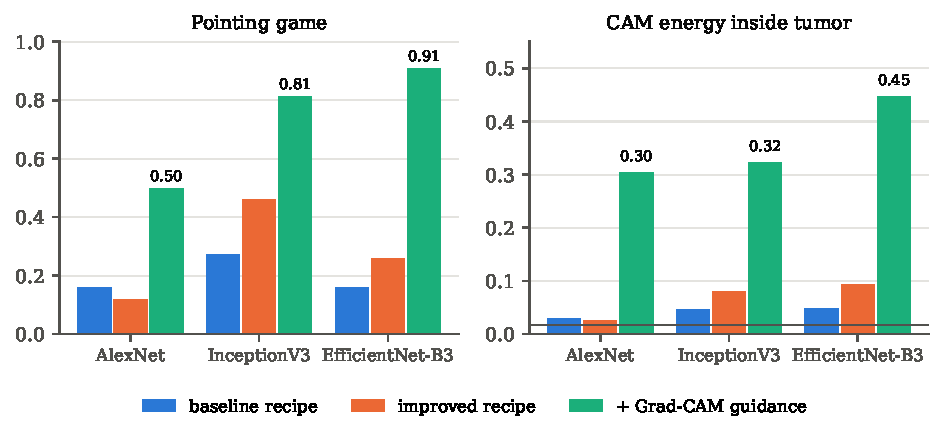
\includegraphics[width=0.9\linewidth]{figures/gradcam_metrics.pdf}
\caption{Pointing game and Grad-CAM energy inside the tumor (4 classes, all folds). The horizontal line in the right
panel is the chance level of a uniform map (0.017).}
\label{fig:gcmetrics}
\end{figure}

\begin{figure}[H]
\centering
\begin{subfigure}{0.66\linewidth}
  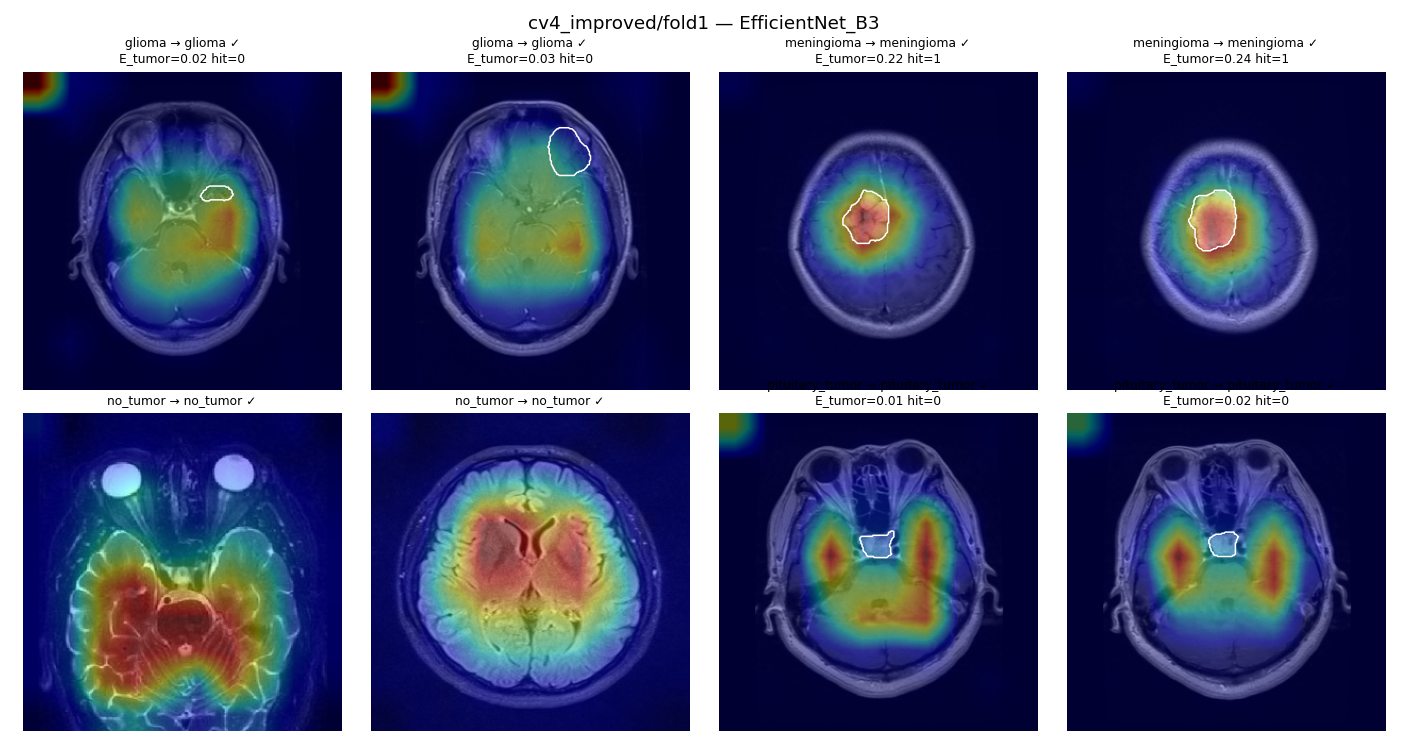
\includegraphics[width=\linewidth]{figures/cam_cv4_improved_effnet.png}
  \caption{improved recipe}
\end{subfigure}\\[4pt]
\begin{subfigure}{0.66\linewidth}
  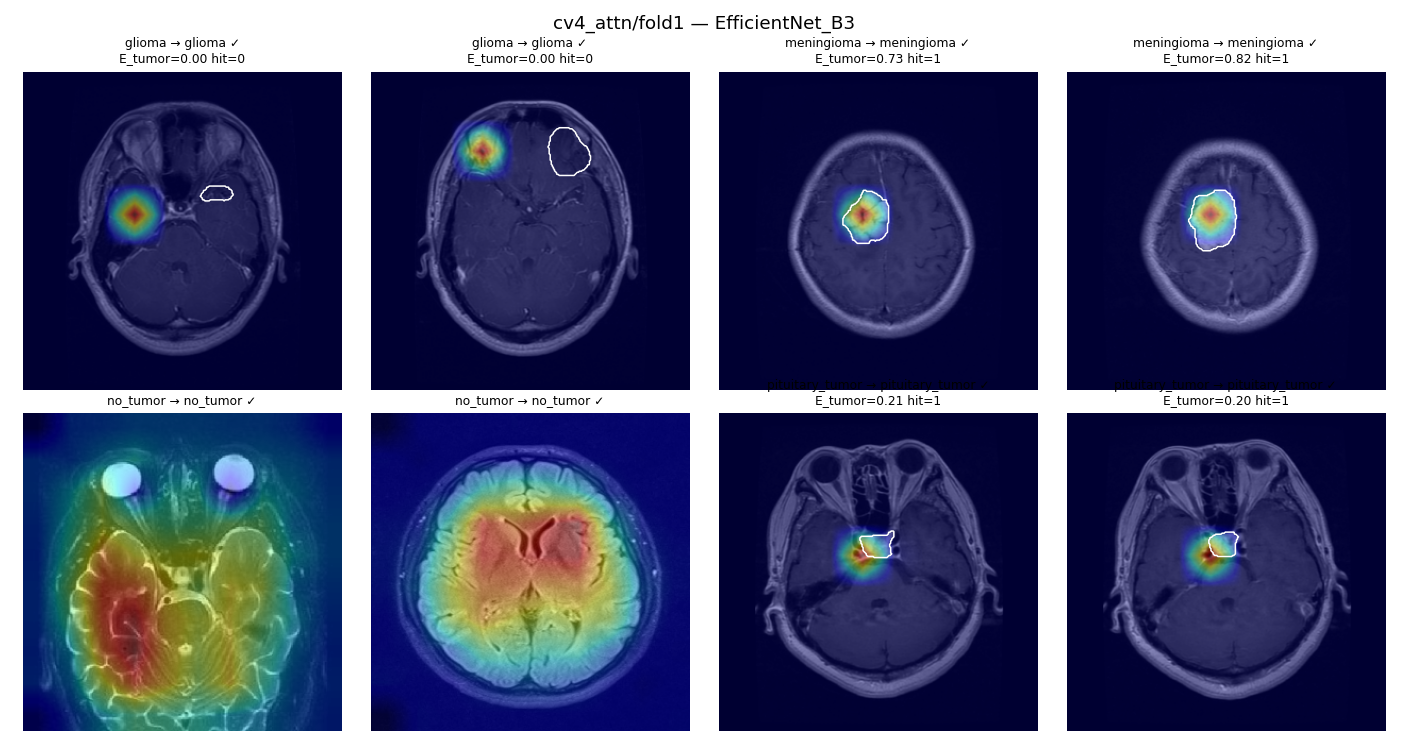
\includegraphics[width=\linewidth]{figures/cam_cv4_attn_effnet.png}
  \caption{+ Grad-CAM guidance}
\end{subfigure}
\caption{EfficientNet-B3 Grad-CAM on the same held-out images (fold 1, two per class). White contour: ground-truth
tumor; title: true $\rightarrow$ predicted class, energy in tumor and pointing hit.}
\label{fig:cams}
\end{figure}

\paragraph{Localisation.} Guidance changes where the networks look (Table~\ref{tab:gradcam}, Fig.~\ref{fig:gcmetrics},
Fig.~\ref{fig:cams}). EfficientNet-B3's Grad-CAM maximum lands on the tumor in 91\,\% of tumor images (from 26\,\%),
with 45\,\% of its mass on the tumor (26$\times$ chance) and 75\,\% within the dilated tumor region. InceptionV3 rises
from 0.46 to 0.81. The final refit models keep this localisation (EfficientNet-B3: pointing 0.898, energy 0.449;
InceptionV3: 0.814, 0.334).

\paragraph{Accuracy.} On three classes, guidance improves InceptionV3 from \pmstd{95.5}{2.2} to \pmstd{96.5}{1.5}\,\%
and EfficientNet-B3 from \pmstd{95.5}{1.7} to \pmstd{96.7}{0.9}\,\% (Fig.~\ref{fig:acc}). The gain concentrates on the
hardest class: meningioma recall rises from 0.895 to 0.922 (Table~\ref{tab:perclass}). AlexNet gains localisation
(pointing $0.12\rightarrow0.50$) but not accuracy, and its Grad-CAM is blank on about half the images.

\begin{figure}[H]
\centering
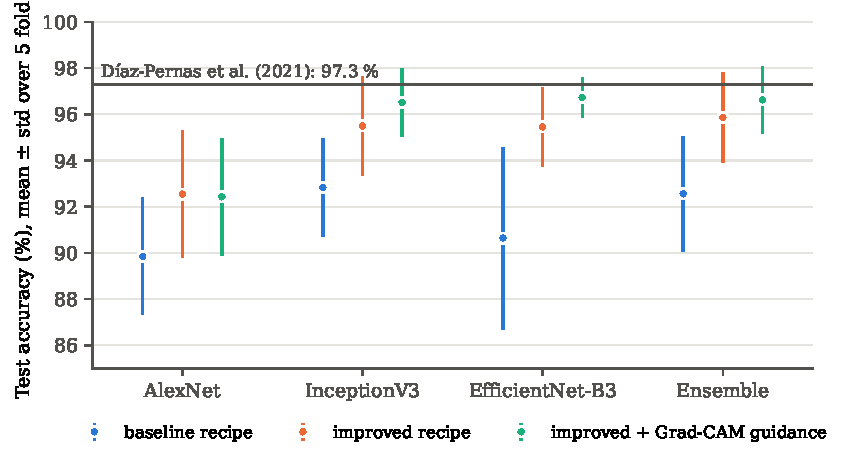
\includegraphics[width=0.85\linewidth]{figures/accuracy_cv3.pdf}
\caption{3-class accuracy (3 training folds) of the baseline recipe, the improved recipe and Grad-CAM guidance; the
ensemble averages AlexNet, InceptionV3 and EfficientNet-B3. The line marks Díaz-Pernas et al.~\cite{diazpernas2021}.}
\label{fig:acc}
\end{figure}

\paragraph{Ablation: loss formulation.} Our first formulation penalised $\sum\mathrm{CAM}\odot(1-M_{\mathrm{dil}})/\sum\mathrm{CAM}$.
This is identical to Eq.~\eqref{eq:guided} whenever the Grad-CAM has positive mass, but it assigns zero loss to a blank
Grad-CAM. AlexNet exploited this: its attention loss fell to 0.003 while all its test Grad-CAMs were blank, with unchanged
accuracy (93.3\,\%). Writing the loss as $1-\text{inside}$ makes a blank map the worst case. The first-generation guided
InceptionV3 and EfficientNet-B3 runs (Fig.~\ref{fig:acc}, Table~\ref{tab:gradcam}) used the first form, with blank
Grad-CAMs on only 4--14\,\% of images. All later runs (Sections~\ref{sec:ablations}--\ref{sec:final}) use
Eq.~\eqref{eq:guided}.

% ──────────────────────────────────────────────────────────────────────────────
\section{Ablations}\label{sec:ablations}

All development runs are guided, use 3 training folds and are ranked by pooled validation accuracy
(Table~\ref{tab:ablations}).

\begin{table}[H]
\centering\small
\caption{Development runs, 3 classes. Validation: pooled over the 5 validation folds. Test: mean\,$\pm$\,std over the
5 test folds. Three numbers separated by slashes are seeds 42 / 1 / 2.}
\label{tab:ablations}
\resizebox{\linewidth}{!}{%
\begin{tabular}{@{}lll@{}}
\toprule
Configuration & Validation (\%) & Test (\%) \\
\midrule
EfficientNet-B3, 300\,px, no guidance (improved recipe) & -- & \pmstd{95.45}{1.71} \\
EfficientNet-B3, 300\,px & 97.13 / 96.93 / 96.90 & 96.46 / 96.35 / 96.30 \\
EfficientNet-B3, 300\,px, EMA weights (0.998) & 96.34 & \pmstd{96.19}{1.28} \\
EfficientNet-B3, 448\,px & -- & \pmstd{96.46}{1.85} \\
InceptionV3, 299\,px & 96.41 / 96.80 / 96.61 & 96.03 / 96.65 / 95.53 \\
InceptionV3, 448\,px & -- & \pmstd{96.09}{1.02} \\
ConvNeXt-T, 384\,px, EMA & 97.10 / 97.13 / 97.00 & 96.17 / 96.65 / 96.24 \\
EfficientNetV2-S, 384\,px, EMA & 96.48 / 96.54 / 96.61 & 96.62 / 96.11 / 96.06 \\
Tumor-region EfficientNet-B3, context $2\times$ & 95.20 / 95.01 / 94.35 & 94.42 / 93.78 / 93.94 \\
Tumor-region EfficientNet-B3, context $3\times$ & 94.81 & \pmstd{94.06}{1.93} \\
Tumor-region ConvNeXt-T, context $2\times$, 384\,px, EMA & 94.45 & \pmstd{94.11}{1.29} \\
\bottomrule
\end{tabular}}
\end{table}

\begin{itemize}
  \item \textbf{Backbone, EMA, resolution.} ConvNeXt-T and EfficientNetV2-S at 384\,px, EMA weights and 448\,px inputs
        all stay within $\pm0.5$ points of EfficientNet-B3 at 300\,px. The bottleneck is not model capacity.
  \item \textbf{Seeds.} The test accuracy of one configuration varies by up to 1.1 points across seeds (InceptionV3),
        as large as many differences between configurations. This motivates selecting and averaging over seeds.
  \item \textbf{Tumor-region crops.} Alone they are 2 points weaker than full images. Small context ($2\times$) is better
        than $3\times$, and EfficientNet-B3 is better than ConvNeXt-T. They make different errors, however
        (Section~\ref{sec:final}).
\end{itemize}

% ──────────────────────────────────────────────────────────────────────────────
\section{Final model}\label{sec:final}

\begin{table}[H]
\centering\small
\caption{Ensembles (uniform average, 3 seeds per configuration). The configuration subset was selected on validation
(top row in bold); the refit rows are evaluated on test once.}
\label{tab:final}
\begin{tabular}{@{}llcc@{}}
\toprule
Ensemble & Training data & Validation (\%) & Test (\%) \\
\midrule
EfficientNet-B3 + InceptionV3 (6 models) & 3 folds & 97.26 & -- \\
\best{+ tumor-region EfficientNet-B3 (9 models)} & 3 folds & \best{97.78} & \pmstd{97.18}{1.22} \\
\midrule
Refit EfficientNet-B3 (3 models) & 4 folds & -- & \pmstd{97.14}{0.99} \\
Refit InceptionV3 (3 models) & 4 folds & -- & \pmstd{96.99}{1.17} \\
Refit tumor-region EfficientNet-B3 (3 models) & 4 folds & -- & \pmstd{94.54}{0.92} \\
Refit without tumor-region models (6 models, ablation) & 4 folds & -- & \pmstd{97.37}{1.05} \\
\best{Refit, selected ensemble (9 models)} & 4 folds & -- & \best{\pmstd{97.64}{1.12}} \\
\bottomrule
\end{tabular}
\end{table}

\begin{figure}[H]
\centering
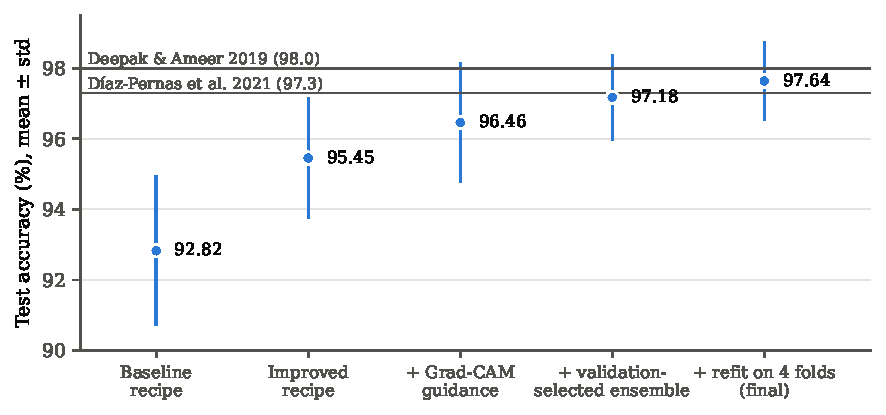
\includegraphics[width=0.9\linewidth]{figures/progression.pdf}
\caption{Test accuracy (3 classes, patient-wise 5-fold, mean $\pm$ std) along the method: baseline recipe
(InceptionV3), improved recipe and Grad-CAM guidance (EfficientNet-B3), validation-selected 9-model ensemble, and its
refit on four folds.}
\label{fig:progression}
\end{figure}

Among all $2^5-1$ subsets of the five configurations (EfficientNet-B3, InceptionV3, ConvNeXt-T, EfficientNetV2-S,
tumor-region EfficientNet-B3), validation selects \emph{EfficientNet-B3 + InceptionV3 + tumor-region EfficientNet-B3}
(Table~\ref{tab:final}). The tumor-region models, although weaker alone, add +0.5 points on validation and +0.3 on test.
Refitting on four folds adds +0.35 to +0.65 points to every configuration and +0.46 to the ensemble. The final
ensemble reaches \best{\pmstd{97.64}{1.12}\,\%} (pooled 97.58\,\%, macro-F1 97.24\,\%; per fold 99.26, 97.20, 97.38,
98.09, 96.27).

\begin{table}[H]
\centering\small
\caption{Pooled per-class recall, 3 classes. Rows 1--3: EfficientNet-B3 trained on 3 folds.}
\label{tab:perclass}
\begin{tabular}{@{}lccc@{}}
\toprule
Model & Glioma & Meningioma & Pituitary \\
\midrule
baseline recipe   & 0.907 & 0.818 & 0.969 \\
improved recipe   & 0.968 & 0.895 & 0.977 \\
+ guidance        & 0.978 & 0.922 & 0.984 \\
\best{final ensemble} & \best{0.985} & \best{0.941} & \best{0.988} \\
\midrule
Díaz-Pernas et al.~\cite{diazpernas2021} & 0.99 & 0.93 & 0.98 \\
\bottomrule
\end{tabular}
\end{table}

\begin{table}[H]
\centering\small
\caption{3-class accuracy on the Figshare dataset under patient-wise cross-validation.}
\label{tab:lit}
\resizebox{\linewidth}{!}{%
\begin{tabular}{@{}llll@{}}
\toprule
Work & Method & Protocol & Accuracy \\
\midrule
Cheng et al.\ 2015~\cite{cheng2015} & tumor-region augmentation, BoW + SVM & patient-wise 5-fold & 91.28\,\% \\
Anaraki et al.\ 2019 (as reported in~\cite{diazpernas2021}) & CNN + genetic algorithm & 5-fold & 94.2\,\% \\
Díaz-Pernas et al.\ 2021~\cite{diazpernas2021} & multiscale CNN & patient-wise 5-fold & 97.3\,\% \\
Deepak \& Ameer 2019~\cite{deepak2019} & GoogLeNet features + SVM/KNN & patient-level 5-fold & 98\,\% \\
\midrule
This work, single EfficientNet-B3 + guidance (refit, mean of 3 seeds) & fine-tuned CNN & patient-wise 5-fold & 97.01\,\% \\
\textbf{This work, final ensemble} & \textbf{9 guided CNNs incl.\ tumor-region models} & \textbf{patient-wise 5-fold} & \best{97.64\,\%} \\
\bottomrule
\end{tabular}}
\end{table}

The final ensemble is 0.34 points above Díaz-Pernas et al.~\cite{diazpernas2021}, the closest published work (same
dataset, protocol and classification+segmentation scope), and 0.36 points below Deepak and Ameer~\cite{deepak2019}
(Table~\ref{tab:lit}). Both margins are smaller than the fold-to-fold standard deviation (1.1 points), so the honest
summary is \emph{on par with the best published results}. Its meningioma recall (0.941) is the highest of the three.

% ──────────────────────────────────────────────────────────────────────────────
\section{Segmentation}\label{sec:seg}

\begin{table}[H]
\centering\small
\caption{Mask R-CNN, patient-wise 5-fold CV (mean\,$\pm$\,std). Misses count as IoU\,=\,Dice\,=\,0; specificity is
measured on the 395 healthy scans.}
\label{tab:seg}
\resizebox{\linewidth}{!}{%
\begin{tabular}{@{}lcccccc@{}}
\toprule
Threshold & Precision & Recall & Specificity & F1 & Mean IoU & Mean Dice \\
\midrule
0.4 & \pmstd{0.967}{0.006} & \pmstd{0.955}{0.008} & \pmstd{0.749}{0.058} & \pmstd{0.961}{0.002} & \pmstd{0.682}{0.022} & \pmstd{0.757}{0.020} \\
0.3 (tuned on val.) & \pmstd{0.958}{0.008} & \pmstd{0.967}{0.005} & \pmstd{0.673}{0.075} & \pmstd{0.963}{0.004} & \pmstd{0.686}{0.021} & \best{\pmstd{0.763}{0.020}} \\
\bottomrule
\end{tabular}}
\end{table}

Mask R-CNN~\cite{maskrcnn} (ResNet-50 FPN, COCO initialisation, two classes, healthy scans with empty targets) is trained
per fold with SGD, cosine schedule and gradient clipping. The checkpoint is selected by validation Dice and the score
threshold by validation F1 (Table~\ref{tab:seg}). It detects 95--97\,\% of tumors with mean Dice 0.76, but a quarter to a
third of healthy scans receive a false detection. Díaz-Pernas et al.~\cite{diazpernas2021} report Dice 0.828 with a
pixel-classification CNN, so segmentation is the stage with the larger gap to the literature. Its out-of-fold boxes
drive the tumor-region classifier of Section~\ref{sec:roi}.

% ──────────────────────────────────────────────────────────────────────────────
\section{Limitations}
\begin{itemize}
  \item The margins to the published results are within one standard deviation of the fold-to-fold spread.
  \item Configurations and the ensemble were selected on validation folds and fixed before the refit. However, test
        accuracies of development candidates were computed and inspected alongside validation accuracies during the
        study, so the development-run test numbers are not fully blind.
  \item Grad-CAM at the last block is coarse ($8\times8$--$13\times13$) and reflects one layer and one explanation method.
  \item The 4-class setting relies on healthy scans from another source (Finding~3).
  \item 2D slices only; no external test set and no clinical validation.
\end{itemize}

\section{Conclusion}
Grad-CAM, measured against tumor masks, shows that accurate brain-tumor classifiers largely ignore the tumor. Using the
masks as a training signal for the Grad-CAM fixes this (pointing game $0.26\rightarrow0.91$) and improves accuracy by
1.0--1.3 points with no test-time cost. Combined with tumor-region classifiers on out-of-fold Mask R-CNN crops,
validation-only ensemble selection and refitting on 80\,\% of the data, the pipeline reaches
\pmstd{97.64}{1.12}\,\% under the official patient-wise protocol. This exceeds the closest published result (97.3\,\%)
and is on par with the best (98\,\%). Larger backbones, EMA and higher resolution did not help; better grounding,
complementary views of the tumor and more training data did.

\section*{Reproducibility}
All experiments are scripts in \texttt{scripts/}, run on one NVIDIA RTX PRO 5000 (48\,GB) with Python 3.10, PyTorch
2.14.1, torchvision 0.29.1 and Albumentations 2.0.8. Every run stores its configuration, history and validation/test
probabilities as JSON in \texttt{results/}. \texttt{scripts/select\_ensemble.py}, \texttt{scripts/summarize.py} and
\texttt{scripts/make\_report\_figures.py} regenerate every table and figure of this report from those files.

\begin{thebibliography}{99}\small
\bibitem{figshare} J.~Cheng. Brain tumor dataset. figshare, dataset 1512427.
  \url{https://doi.org/10.6084/m9.figshare.1512427}
\bibitem{cheng2015} J.~Cheng, W.~Huang, S.~Cao, R.~Yang, W.~Yang, Z.~Yun, Z.~Wang, Q.~Feng. Enhanced performance of brain
  tumor classification via tumor region augmentation and partition. \emph{PLoS ONE} 10(10): e0140381, 2015.
\bibitem{bhuvaji} S.~Bhuvaji, A.~Kadam, P.~Bhumkar, S.~Dedge, S.~Kanchan. Brain Tumor Classification (MRI). Kaggle, 2020.
\bibitem{deepak2019} S.~Deepak, P.~M.~Ameer. Brain tumor classification using deep CNN features via transfer learning.
  \emph{Computers in Biology and Medicine} 111: 103345, 2019.
\bibitem{diazpernas2021} F.~J.~Díaz-Pernas, M.~Martínez-Zarzuela, M.~Antón-Rodríguez, D.~González-Ortega. A deep learning
  approach for brain tumor classification and segmentation using a multiscale convolutional neural network.
  \emph{Healthcare} 9(2): 153, 2021.
\bibitem{alexnet} A.~Krizhevsky, I.~Sutskever, G.~E.~Hinton. ImageNet classification with deep convolutional neural
  networks. \emph{NeurIPS}, 2012.
\bibitem{inception} C.~Szegedy, V.~Vanhoucke, S.~Ioffe, J.~Shlens, Z.~Wojna. Rethinking the Inception architecture for
  computer vision. \emph{CVPR}, 2016.
\bibitem{efficientnet} M.~Tan, Q.~V.~Le. EfficientNet: Rethinking model scaling for convolutional neural networks.
  \emph{ICML}, 2019.
\bibitem{efficientnetv2} M.~Tan, Q.~V.~Le. EfficientNetV2: Smaller models and faster training. \emph{ICML}, 2021.
\bibitem{convnext} Z.~Liu, H.~Mao, C.-Y.~Wu, C.~Feichtenhofer, T.~Darrell, S.~Xie. A ConvNet for the 2020s.
  \emph{CVPR}, 2022.
\bibitem{maskrcnn} K.~He, G.~Gkioxari, P.~Dollár, R.~Girshick. Mask R-CNN. \emph{ICCV}, 2017.
\bibitem{gradcam} R.~R.~Selvaraju, M.~Cogswell, A.~Das, R.~Vedantam, D.~Parikh, D.~Batra. Grad-CAM: Visual explanations
  from deep networks via gradient-based localization. \emph{ICCV}, 2017.
\bibitem{pointinggame} J.~Zhang, S.~A.~Bargal, Z.~Lin, J.~Brandt, X.~Shen, S.~Sclaroff. Top-down neural attention by
  excitation backprop. \emph{IJCV} 126: 1084--1102, 2018.
\bibitem{ross2017} A.~S.~Ross, M.~C.~Hughes, F.~Doshi-Velez. Right for the right reasons: Training differentiable models
  by constraining their explanations. \emph{IJCAI}, 2017.
\bibitem{caruana2004} R.~Caruana, A.~Niculescu-Mizil, G.~Crew, A.~Ksikes. Ensemble selection from libraries of models.
  \emph{ICML}, 2004.
\end{thebibliography}

\end{document}
